\documentclass[12pt]{article}
\usepackage{graphicx}
\usepackage{tikz}
\usetikzlibrary{positioning}

\begin{document}

\section{Connecting nodes}

Try out the \textbackslash{}path let command to place a new node relative to \textbf{a} and \textbf{b}!
\vspace{1em}

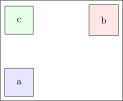
\includegraphics{_img_src/path-let.pdf}

\vspace{1em}
\hrule 
\vspace{1em}

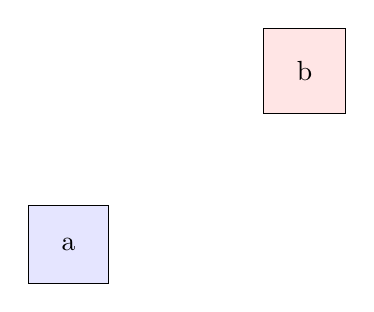
\begin{tikzpicture}

    \node[draw, inner sep=12pt, fill=blue!10] (a) {a};
    \node[draw, inner sep=12pt, fill=red!10] (b) at (3, 2.2) {b};

    %%%%%%%%%%%%%%%%%%%%%
    % Add your code here
    %%%%%%%%%%%%%%%%%%%%%
    
\end{tikzpicture}

\end{document}